%%%%%%%%%%%%%%%%%%%%%%%%%%%%%%%%%%%%%%%%%%%%%%
%		Markros für Titel etc
%%%%%%%%%%%%%%%%%%%%%%%%%%%%%%%%%%%%%%%%%%%%%%
\newcommand{\thefaculty}{Hochschule Hannover -- Fakultät IV}

\newcommand{\theauthor}{Simon Beckstein}
\newcommand{\thetitle}{Bachelorarbeit}
\newcommand{\thetopic}{Exemplarische Untersuchung der Wartbarkeit von Webanwendungen unter Einsatz des Google Web Toolkit.}
\newcommand{\thepublisher}{\thefaculty\\Angewandte Informatik (BIN)\\Prof. Dr. Robert Garmann}
\newcommand{\theversion}{Stand vom \today}


\date{Sommersemester 2012}

\documentclass[
	paper=a4,
	fontsize=12pt,
	bibliography=totoc,
	listof=totoc,
%	draft,
	twoside,
]{scrreprt}

%%%%%%%%%%%%%%%%%%%%%%%%%%%%%%%%%%%%%%%%%%%%%%
%		Basis Präambel
%%%%%%%%%%%%%%%%%%%%%%%%%%%%%%%%%%%%%%%%%%%%%%

\usepackage[ngerman]{babel}
\usepackage[utf8]{inputenc}
\usepackage[T1]{fontenc}
\usepackage[babel,german=quotes]{csquotes}


%%%%%%%%%%%%%%%%%%%%%%%%%%%%%%%%%%%%%%%%%%%%%%
%	Einstellungen der Titelsetie
%%%%%%%%%%%%%%%%%%%%%%%%%%%%%%%%%%%%%%%%%%%%%%

\title{\thetitle}
\subtitle{\thetopic}
\author{\theauthor}
\publishers{\thepublisher}



%%%%%%%%%%%%%%%%%%%%%%%%%%%%%%%%%%%%%%%%%%%%%%
%		Seitenabmessungen
%%%%%%%%%%%%%%%%%%%%%%%%%%%%%%%%%%%%%%%%%%%%%%

\usepackage[
	left=2.5cm,
	right=2.5cm,
	top=2.5cm,
	bottom=2.5cm,
	bindingoffset=1cm,
	includehead,
	includefoot
]{geometry}

%%%%%%%%%%%%%%%%%%%%%%%%%%%%%%%%%%%%%%%%%%%%%%
%		Parameterlose Packete
%%%%%%%%%%%%%%%%%%%%%%%%%%%%%%%%%%%%%%%%%%%%%%

\usepackage{
%	fancyhdr,
	graphicx,
%	amssymb,
%	makeidx,
	listings,
	lmodern,
	wrapfig,
	subfig,
	blindtext,
	csquotes,
	lastpage,
	paralist,
	color,
	xcolor,
	MnSymbol,
	pdfpages,
	todonotes,
}

\shorthandoff{"}

%%%%%%%%%%%%%%%%%%%%%%%%%%%%%%%%%%%%%%%%%%%%%%
%		Einstellungen für Listings
%%%%%%%%%%%%%%%%%%%%%%%%%%%%%%%%%%%%%%%%%%%%%%

\definecolor{dkgreen}{rgb}{0,0.6,0}
\definecolor{gray}{rgb}{0.5,0.5,0.5}
\definecolor{mauve}{rgb}{0.58,0,0.82}
 
\lstset{ %
	%extendedchars=\true,
	%inputencoding=utf8,
	floatplacement=htb,
	language=Java,
	basicstyle=\footnotesize\ttfamily,	%quelltext ist etwas kleiner als normaler text
	numbers=left,
	numberstyle=\tiny\color{gray},		%kleine, graue Zeilennummern
	stepnumber=1,
	numbersep=5pt,                  	%Entfernung der Zeilennummern zum Code
	backgroundcolor=\color{white},
	showspaces=false,               	%keine Unterstriche für Leerzeichen
	showstringspaces=false,         	%auch nicht für Strings
	showtabs=false,                 	%und nicht für tabs
	frame=single,
	rulecolor=\color{black}, 			%Achtung muss gesetzt sein, weils sonst bunte
										%rahmen gibt.
	tabsize=2,
	captionpos=b,						%Beschriftung unter dem Code
	breaklines=true,					%zeilen Umbrechen, ragen sonst über Rand hinaus
	breakatwhitespace=false, 			%hartes Umbrechen, folgende Zeilen fügen aber
										%entsprechende Markierungen hinzu
	prebreak=\raisebox{0ex}[0ex][0ex]{\color{black}\ensuremath{\rhookswarrow}},
	postbreak=\raisebox{0ex}[0ex][0ex]{\color{black}\ensuremath{\rcurvearrowse}},
	title=\lstname,						%Zeigt Dateinamen wenn keine caption angegeben
	keywordstyle=\color{blue},			%blaue Keywörter, wie void oder null
	commentstyle=\color{dkgreen},		%grüne Kommentare
	stringstyle=\color{mauve}, 			%und die Strings 
	escapeinside={\%*}{*)},				%ermöglicht kommentare im Listing mit %
	morekeywords={create,Void},			%zusätzliche keywords
}

%sorgt dafür, dass man in listings auch umlaute benutzen kann. dies
%geht leider nicht wenn die dokumente utf8 kodiert sind. verwendet man
%latin1, gibt es keine probleme.
\lstset{literate=%
	{Ö}{{\"O}}1
	{Ä}{{\"A}}1
	{Ü}{{\"U}}1
	{ß}{{\ss}}2
	{ü}{{\"u}}1
	{ä}{{\"a}}1
	{ö}{{\"o}}1
}

%irgend ein komisches Makro, was dafür sorgt, dass über lstinline eingefügter
%code die selbe textgröße hat wie der normale text, weil
%normale listings etwas kleiner in der schriftgröße sind
%http://www.latex-community.org/forum/viewtopic.php?f=5&t=2072
\makeatletter
	\lst@AddToHook{TextStyle}{\let\lst@basicstyle\normalsize\ttfamily}
\makeatother


%%%%%%%%%%%%%%%%%%%%%%%%%%%%%%%%%%%%%%%%%%%%%%
%		Einstellungen für PDF
%%%%%%%%%%%%%%%%%%%%%%%%%%%%%%%%%%%%%%%%%%%%%%

\usepackage[colorlinks=true,
	breaklinks=false,
	linktocpage=false,
	linkcolor=black,
	citecolor=black,
	filecolor=black,
	urlcolor=blue,
	frenchlinks=false,
	bookmarks=true,
	bookmarksopen=true,
	bookmarksopenlevel=3,
	plainpages=false,
	pdfpagelabels=true,
	pdftitle={\thetitle},
	pdfauthor=\theauthor,
	pdfsubject={\thetopic},
]{hyperref}

\pdfinfo{
    /Author (\theauthor)
    /Title (\thetitle)
    /Subject (\thetopic)
}


%%%%%%%%%%%%%%%%%%%%%%%%%%%%%%%%%%%%%%%%%%%%%%
%		Header/Footer der Seiten
%%%%%%%%%%%%%%%%%%%%%%%%%%%%%%%%%%%%%%%%%%%%%%

\usepackage[
	headsepline,
	footsepline,
	automark,
]{scrpage2}

% Festlegung Kopf- und Fußzeile     
\defpagestyle{meinstil}{%
	{\headmark \hfill}
	{\hfill \headmark}
	{\hfill \headmark\hfill }
	(\textwidth,.4pt)
}{%
	(\textwidth,.4pt)
	{\pagemark\hfill\thefaculty}
	{\theauthor\hfill\pagemark}
	{\hfill\pagemark} 
}
\pagestyle{meinstil} 



%%%%%%%%%%%%%%%%%%%%%%%%%%%%%%%%%%%%%%%%%%%%%%
%		Eigene Befehle
%%%%%%%%%%%%%%%%%%%%%%%%%%%%%%%%%%%%%%%%%%%%%%





\begin{document}


%%%%%%%%%%%%%%%%%%%%%%%%%%%%%%%%%%%%%%%%%%%%%%
%	Titelseite und Verzeichnisse
%%%%%%%%%%%%%%%%%%%%%%%%%%%%%%%%%%%%%%%%%%%%%%


\maketitle
\tableofcontents
\newpage
\lstlistoflistings
\newpage
\listoffigures

%\begin{minipage}{\textwidth}\listoftables\end{minipage}


\chapter*{Beteiligte}
\begin{minipage}{\textwidth}

	\section*{Erstprüfer}
	\textbf{Prof. Dr. Robert Garmann}\\
	Ricklinger Stadtweg 120\\
	30459  Hannover\\
	
	Raum: 303\\
	Tel.: +49 511 9296-1832\\
	E-Mail: \href{mailto:robert.garmann@fh-hannover.de}{robert.garmann@fh-hannover.de}
	
	\section*{Zweitprüfer}
	\textbf{Prof. Dr. Ralf Bruns}\\
	Ricklinger Stadtweg 120\\
	30459  Hannover\\
	
	Raum: 354\\
	Tel.: +49 511 9296-1817\\
	E-Mail: \href{mailto:ralf.bruns@fh-hannover.de}{ralf.bruns@fh-hannover.de}
	
	
	\section*{Autor}
	\textbf{Simon Beckstein}\\
	Lohgerberstr. 8\\
	31303 Burgdorf\\
	
	Matrikel Nr.: 1114284\\
	E-Mail: \href{mailto:simon.beckstein@stud.fh-hannover.de}{simon.beckstein@stud.fh-hannover.de}
\end{minipage}


\chapter*{Erklärung der Selbstständigkeit}
\begin{center}
	\framebox[0.9\textwidth][c]{
		\begin{minipage}{0.8\textwidth} 
			\vspace*{2ex}
			\begin{center} 
				\bfseries Selbständigkeitserklärung 
			\end{center}
			\input{erklaerung-text.txt}
			\vspace*{30ex}
													
														%unterstrichene Leerzeichen
			\underline{Burgdorf, \today} \hfill \underline{\ \ \ \ \ \ \ \ \ \ \ \ \ \ \ \ \ \ \ \ \ \ \ \ \ \ \ \ \ \ \ \ \ \ \ \ }
			
			Ort, Datum \hfill Unterschrift
			\vspace*{2ex}		
		\end{minipage}		
	}
\end{center}
	

%%%%%%%%%%%%%%%%%%%%%%%%%%%%%%%%%%%%%%%%%%%%%%
%	Hauptarbeit
%%%%%%%%%%%%%%%%%%%%%%%%%%%%%%%%%%%%%%%%%%%%%%


\cleardoublepage
\chapter{Einleitung}
\cleardoublepage
\chapter{Hauptteil}
\section{Figures und Floats}
\begin{wrapfigure}{L}{0.46\textwidth}
  \centering
	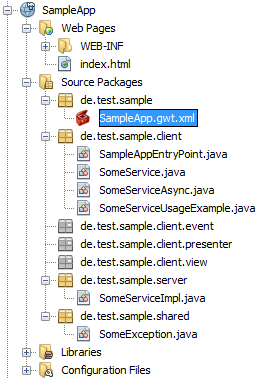
\includegraphics[]{figures/SampleAppProjektbaum}
    \caption{Projektbaum eines GWT Moduls}    
  \label{fig:projektbaum}
\end{wrapfigure}

\blindtext[2]

\begin{figure}[ht]
  \centering
	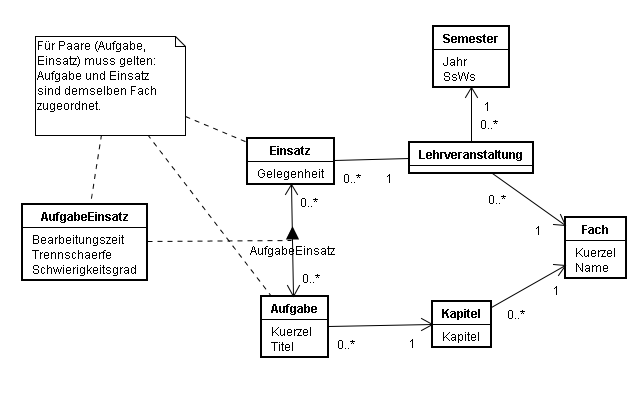
\includegraphics[width=\textwidth]{figures/DomainModel}
    \caption[Domänenmodell der Aufgabenpoolverwaltung]{Domänenmodell der Aufgabenpoolverwaltung.\\ \textbf{Quelle:} Prof. Dr. Robert Garmann}
  \label{fig:domainmodel}
\end{figure}

\begin{wrapfigure}{r}{0.45\textwidth}
  \vspace{-25pt}
  \centering
  \subfloat[Klassiches MVP]{\label{fig:mvp1}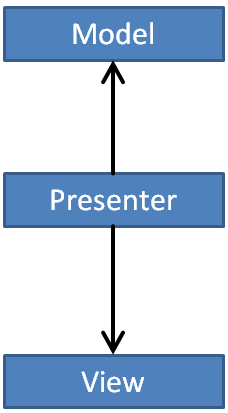
\includegraphics[scale=0.5]{figures/mvp1}}
  \quad
  \subfloat[MVP in der GWT-Architektur]{\label{fig:mvp2}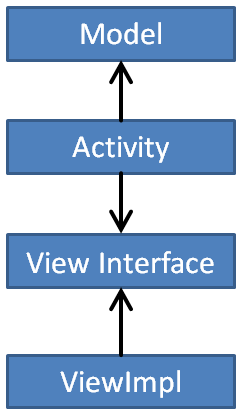
\includegraphics[scale=0.5]{figures/mvp2}}
    \caption{MVP nach \cite{GuUn2010}}
  \label{fig:mvp}  
  \vspace{-15pt}
\end{wrapfigure}

\blindtext[2]

\section{Listings}

Code wird für Java hervorgehoben. Ebenso inline-code wie dieser: \lstinline|public void essen() { System.out.println("esse"); }|

\lstinputlisting[float,label=lst:requestfactory,caption={Verwendung der RequestFactory beim Client\cite{GWT_REQ}}]{code/requestfactory.java}


\lstinputlisting[label=lst:uibinder_xml,language=xml,caption={Die XML-Beschreibung eines einfachen Widgets}]{code/HelloWidgetWorld.ui.xml}

Die Angabe von \lstinline|float| in den Attributen von \lstinline|\lstinputlisting| sorgt dafür, dass Quelltext nicht umgebrochen wird. 


\section{Sonstiges}
\subsection{Listen}
\begin{itemize}
\item eins
\item zwei
\item drei
\end{itemize}

\begin{enumerate}
\item eins
\item zwei
\item drei
\end{enumerate}

\subsection{Definitionen}
\begin{description}
\item[eins] ne zahl
\item[zwei] noch ne zahl
\item[drei] und noch eine
\end{description}

\subsection{Kompakte listen}
Die normalen Auflistungen haben viel whitespace oben und unten und zwischen drin. Mit \texttt{compactitem} kann dieser platz....
\begin{compactitem}
\item eins
\item zwei
\item drei
\end{compactitem}
.... verringert werden

\subsection{Todo Notes}
\todo{Referenz finden} Todonotes sind nützlich um Notizen im Fließtext zu platzieren. Können auch über eine ganze Zeile gehen
\todo[inline]{Test}

\section{Tabellen}
\blindtext
\begin{table}[h]
	\centering
	\begin{tabular}{|l|l|l|}
\hline 
		Metrik 		  &Beschreibung 								&  Brauchbarkeit\\ 
\hline  
		\textbf{WMC}  &Gewichtete Methoden pro Klasse 				&  mäßig 		\\ 
\hline  
		\textbf{DIT}  &Tiefe im Vererbungsbaum 						&  hoch 		\\ 
\hline  
		\textbf{RFC}  &Antwortmenge einer Klasse 					&  hoch 		\\ 
\hline 
		\textbf{NOC}  &Zahl von Unterklassen 						&  hoch 		\\ 
\hline  
		\textbf{LCOM} &Mangel an Zusammenhang zwischen Methoden 	&  niedrig  	\\ 
\hline  
		\textbf{CBO}  &Kopplung zwischen Objektklassen 				&  hoch  		\\ 
\hline 
	\end{tabular} 
	\caption{Kennzahlen nach Chidamber \& Kemerer (aus \cite{Prech1999})}
	\label{tab:metrik}
\end{table}


\begin{table}[h]
	\centering
	\begin{tabular}{lp{6cm}p{6cm}}
		\toprule
		\multicolumn{3}{c}{Chidamber \& Kemerer}\\ 
		\midrule
		\textbf{WMC}  &Anzahl gewichteter Methoden 				&  Weigthed Methods per Class 		\\ 
		\textbf{DIT}  &Tiefe der Vererbungshierarchie  			&  Depth of Inheritance Tree 		\\ 
		\textbf{NOC}  &Anzahl der Unterklassen 					&  Number of Children 				\\ 
		\textbf{CBO}  &Kopplung der Klassen 					&  Coupling Between Object Classes 	\\  
		\textbf{RFC}  &Anzahl potentieller Zielmethoden 		&  Respone for a Class  			\\  
		\textbf{LCOM} &Mangel an Zusammenhalt der Methoden
		 				einer Klasse 							&  Lack of Cohesion in Methods  		\\ 
		\bottomrule
	\end{tabular} 
	\caption{Kennzahlen nach Chidamber \& Kemerer (zusammengetragen aus \cite{Prech1999,Sneed2010,Chidamber1994})}
	\label{tab:ck}
\end{table}


\begin{table}[h]
	\rowcolors{2}{lightgray}{white}
	\centering
	
	\begin{tabular}{lp{6cm}p{6cm}}
		\toprule
		\multicolumn{3}{c}{Chidamber \& Kemerer}\\ 
		\midrule
		\textbf{WMC}  &Anzahl gewichteter Methoden 				&  Weigthed Methods per Class 		\\ 
		\textbf{DIT}  &Tiefe der Vererbungshierarchie  			&  Depth of Inheritance Tree 		\\ 
		\textbf{NOC}  &Anzahl der Unterklassen 					&  Number of Children 				\\ 
		\textbf{CBO}  &Kopplung der Klassen 					&  Coupling Between Object Classes 	\\  
		\textbf{RFC}  &Anzahl potentieller Zielmethoden 		&  Respone for a Class  			\\  
		\textbf{LCOM} &Mangel an Zusammenhalt der Methoden
		 				einer Klasse 							&  Lack of Cohesion in Methods  		\\ 
		\bottomrule
	\end{tabular} 
	\caption{Mit abwechselnden Farben....}
	\label{tab:ck}
\end{table}



\section{Zitate}

Inline-Zitate stehen \enquote{\emph{mitten im Text}} und sind üblicherweise kursiv gedruckt, außerdem sind sie in den Satz eingebunden.

Abgesetzte Zitate werden entweder mit der quote-Umgebung für kurze Zitate gemacht, oder mit der qoutation-Umgebung für längere Zitate

\begin{quote}
Nachts ist es kälter als Draußen
\end{quote}


\begin{quotation}
Hiermit erkläre ich an Eides Statt, dass ich die eingereichte Masterarbeit
				selbständig und ohne fremde Hilfe verfasst, andere als die von mir angegebenen Quellen
				und Hilfsmittel nicht benutzt und die den benutzten Werken wörtlich oder
				inhaltlich entnommenen Stellen als solche kenntlich gemacht habe. 
\end{quotation}

Da diese häufig eine Quellenangabe benötigen und diese häufig unten rechts vom Zitat zu finden ist, habe ich eine aquote-Umgebung aus dem Interwebz eingefügt:

\begin{aquote}{Eidesstattliche Erklärung der Hochschule}
Hiermit erkläre ich an Eides Statt, dass ich die eingereichte Masterarbeit
				selbständig und ohne fremde Hilfe verfasst, andere als die von mir angegebenen Quellen
				und Hilfsmittel nicht benutzt und die den benutzten Werken wörtlich oder
				inhaltlich entnommenen Stellen als solche kenntlich gemacht habe. 
\end{aquote}

\begin{aquote}{Unbekannt}
Nachts ist es kälter als Draußen
\end{aquote}

\cleardoublepage
\chapter{Schluss}

\cleardoublepage

%%%%%%%%%%%%%%%%%%%%%%%%%%%%%%%%%%%%%%%%%%%%%%
%	Anhänge
%%%%%%%%%%%%%%%%%%%%%%%%%%%%%%%%%%%%%%%%%%%%%%

\appendix
\chapter{Anhang}
\cleardoublepage
\chapter{Anhang}
\cleardoublepage

%%%%%%%%%%%%%%%%%%%%%%%%%%%%%%%%%%%%%%%%%%%%%%
%	Literatur
%%%%%%%%%%%%%%%%%%%%%%%%%%%%%%%%%%%%%%%%%%%%%%

\nocite{*}		%auch nicht verwendete literatur ausgeben
\bibliographystyle{alphadin}

\bibliography{literatur}



\end{document}

